% vim:ft=tex
% rubber: module xelatex
\subsection{Camera calibration}
\label{sec:calibration}
For the camera calibration part of the application, we have
implemented the calibration algorithm from \cite{TSAI}, which is a
classical and often cited calibration method. The article encompasses
several different methods of calibration; we are implementing the
method that the article describes as "the monoview non-coplanar
case''. That is, the calibration is performed from a single image
of a calibration object that has calibration points in several (world)
planes.

Our calibration object can be seen in figure~\ref{fig:calib-object}.
It consists of two adjacent faces of a cube, each of which has a
number of circular calibration points. The left face has 35 points,
and the right face 28. The distance between point centres is 1,5
inches. The world coordinate system is chosen to be a right-handed
coordinate system, centred at the bottom corned of the cube, so the
left face corresponds to the YZ plane, and the right face corresponds
to the XZ plane.

\begin{figure}[hb]
  \centering
  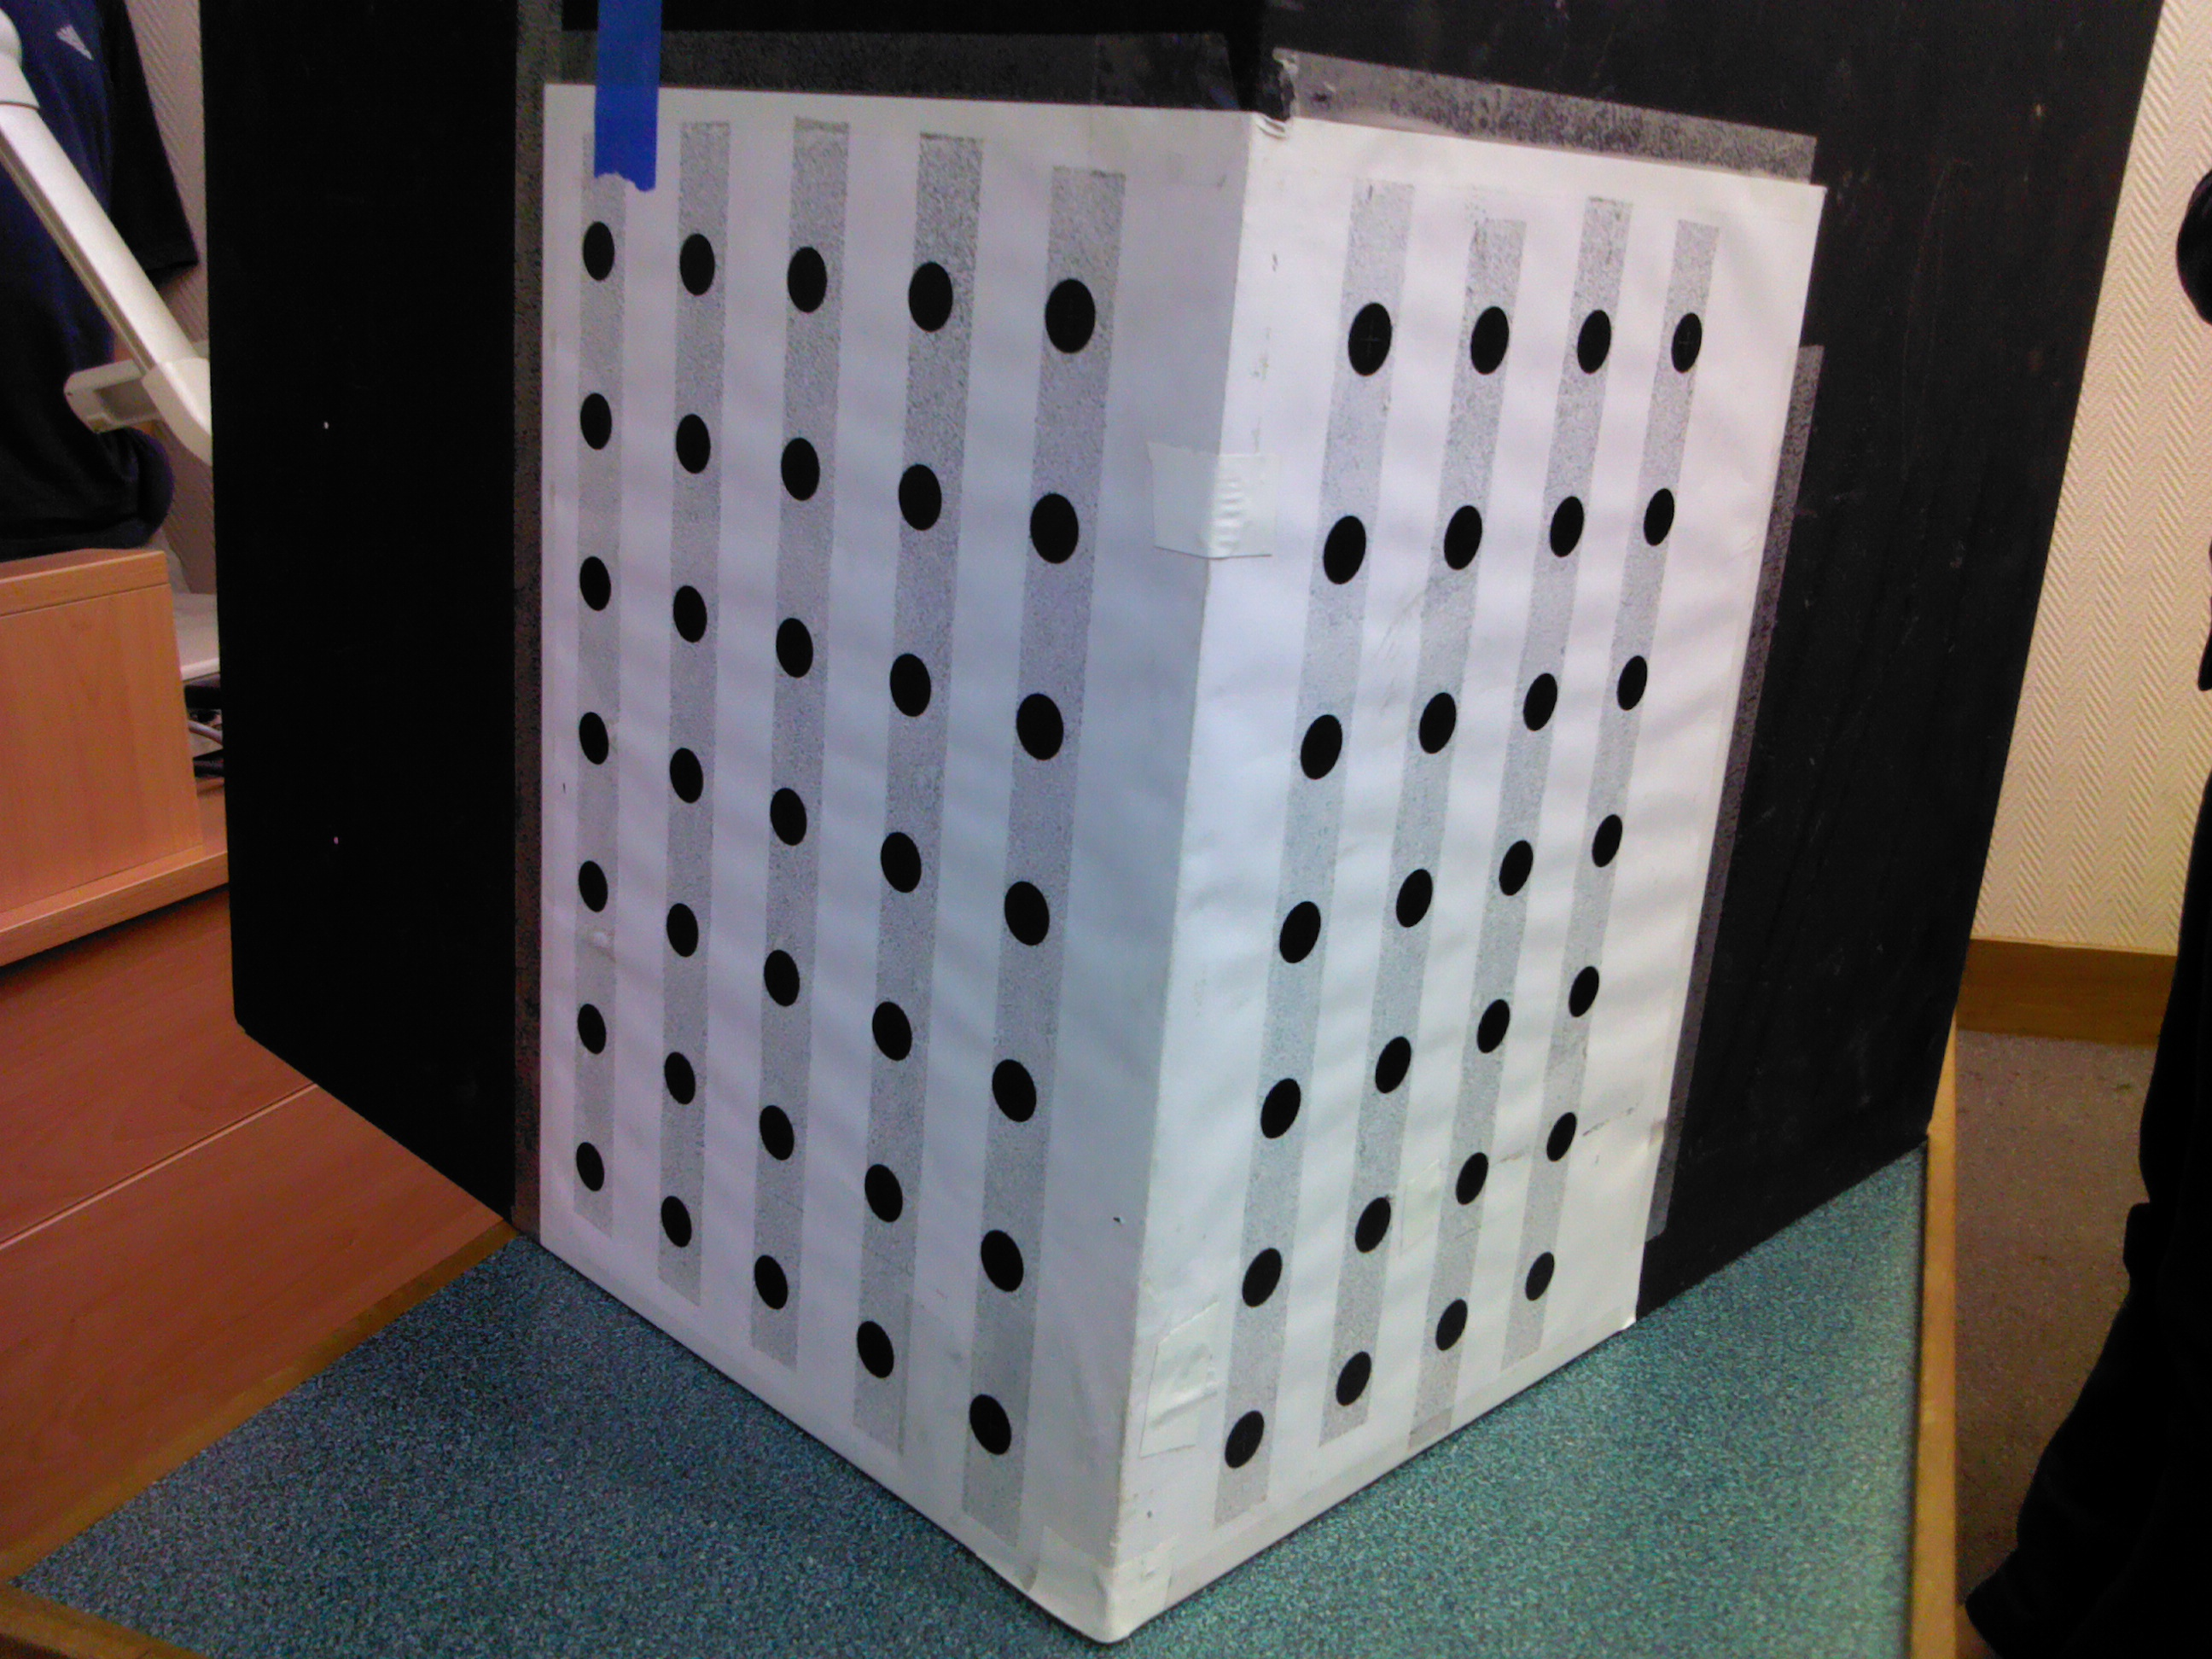
\includegraphics[width=0.7\textwidth]{figures/calibration-object}
  \caption[Calibration object]{Calibration object. The left face has
    35 calibration points (the centres of the circles), and the right
    face has 28. The distance between point centres is 1,5 inches. The
    world coordinate system is chosen to be a right-handed coordinate
    system, centred at the bottom corned of the cube, so the left face
    corresponds to the YZ plane, and the right face corresponds to the
    XZ plane.}
  \label{fig:calib-object}
\end{figure}

\subsubsection{Implementation notes}
The implementation overall follows the procedure laid out in
\cite{TSAI}. However, a few notes on the implementation are
appropriate:

\paragraph{Implemented parts of the algorithm.}
As mentioned, we implement the calibration method that Tsai refers to
as ``the monoview non-coplanar case''. The calibration function derives
the transformation matrix, composed of the rotation matrix, $R$ and
the translation matrix $T$, find the scale factor $s_x$, and the
intrinsic camera values $f$ (focal length) and $\kappa$ (radial
distortion parameter). The radial distortion is calculated as far as
$\kappa_1$. The literature suggests that this is sufficient for
reasonably high accuracy using cameras without significant lens
distortion \cite{algebraic-distortion}.

\paragraph{Mapping of image coordinates to world coordinates.}
The world coordinates of the points are measured manually, in units of
inches. These are given as input to the program in the form of a
space-separated text file. The image coordinate points are found by
first running the SURF feature point extraction algorithm described in
section~\ref{sec:features} on the input image, with a relatively high
threshold value (500). The feature points detected using this
algorithm are shown to the user on a binary image (obtained using
adaptive thresholding -- see the description of the segmentation
algorithms in section~\ref{sec:segmentation}), who then has the option
of removing and adding points.

These user-corrected points are fed to the second stage of the
calibration algorithm. This stage assumes that there are exactly 63
points selected on the image, and furthermore takes as input exactly
63 3D points (corresponding to the 63 circles on the calibration
object). The image points are first corrected to be closer to the
centre of the circle. This is done by flood filling the binary image
from each point with a threshold of 0 (i.e. finding all pixels of the
same colour as the point), and taking the average x and y values from
this region. This means that the user does not have to select points
that are exactly at the centre of the calibration region, but can
click anywhere within it.

Following this correction, the image points are mapped to the real
world coordinate points. This is done by a brute-force algorithm
relying on the fact that
\begin{inparaenum}[(a)]
  \item the right and left faces are entirely disjoint in the
    horizontal direction, i.e. no points on the right face have
    x-coordinates lower than any points on the left face, and
  \item the top and bottom outermost points in each face are the
    points closest to the respective image corners on that side of the
    image.
\end{inparaenum}
This algorithm does impose some limitations on the possible viewing
angles of the calibration object. For example, if the image is rotated
by enough to make the faces overlap in the horizontal direction, the
first assumption breaks down and the image point to world point
mapping fails.

\paragraph{Back-projection.}
To test the error ratio of the calibration, we reverse the direction
of projection, by projecting the rays from the camera through the
image coordinate points onto the corresponding face planes in world
coordinates (taking into account the (reversed) calibration
parameters). This allows us to measure the distance between these
derived world coordinates and the known ones as an error radius.

\paragraph{Implementation problems.}
We have encountered a few problems in our implementation. Primarily,
it was not completely obvious to us that, in going from the coplanar
to the non-coplanar cases, equation (15) in \cite{TSAI} has to be
re-derived from the earlier equation (8b), because the it is no longer
true that $z_w=0$. Also, it proved tricky to get the back-projection
working correctly.

\subsection{Experimental results}
For testing the calibration, we have run the program on four different
pictures of the calibration object, taken with two different cameras.
In this section, we go thnrough the results, first by doing some sanity
checking on the values from observations of the environment, and then
by looking at the errors from the back-projection estimates.

\begin{table}[htb]
  \centering
  \begin{tabular}{c c c c c c}
    \toprule
    \multicolumn{3}{c}{\textbf{Rotation}} & \multicolumn{3}{c}{\textbf{Translation}}\\
    \midrule
    \multicolumn{3}{c}{$R=\begin{bmatrix}0.69 & -0.72 & 0.08\\
    0.14 & 0.25 & 0.96\\
    -0.70 & -0.65 & 0.28\end{bmatrix}$} &
    \multicolumn{3}{c}{$T=\begin{bmatrix}0.00\\-6.76\\-16.80\end{bmatrix}$} \\
    \midrule
    \multicolumn{2}{c}{\textbf{Scaling}} &
    \multicolumn{2}{c}{\textbf{Focal length}} &
    \multicolumn{2}{c}{\textbf{Distortion}}\\
    \midrule
    \multicolumn{2}{c}{$s_x =0.998$} &
    \multicolumn{2}{c}{$f=-2424.61$} &
    \multicolumn{2}{c}{$\kappa_1=-1.76 \cdot 10^{-8}$}\\
    \bottomrule
  \end{tabular}
  \caption[Calibration results]{Calibration results. This is the
    results of calibration for the first image (labelled 160019 in
    figure~\ref{fig:calib-errors}).}
  \label{tbl:calib-results}
\end{table}

One of the results of the calibration can be seen in
table~\ref{tbl:calib-results}. Looking at the translation vector,
according to the calibration, the corner of the calibration object is
just under 17 inches in front of the camera (or camera plane) and just
under 7 inches below it. These figures are roughly consistent with the
distance from which the picture is taken, so the calibration does not
appear to be completely off.

Furthermore, in table~\ref{tbl:focal-lengths} is a comparison
between the focal length results for the four images. From this, it is
apparent that images taken with the same camera have similar focal
lengths, and the focal lengths of images taken with different cameras
are quite different. These two sanity tests together suggest that the
results of the calibration are not completely off.

\begin{table}[h]
  \centering
  \begin{tabular}{c c}
    \toprule
    \textbf{Image} & \textbf{Focal length}\\
    \midrule
    160019 & -2424.61\\
    160027 & -2412.75\\
    0025 & -4887.01\\
    0026 & -4701.72\\
    \bottomrule
  \end{tabular}
  \caption[Focal length values for the test images]{Focal length
    values for the test images. The images are taken pairwise with two
    different cameras; this is reflected in the focal length values,
    in that images taken with the same camera have very similar focal
    lengths, and there is a large variation between the two cameras.}
  \label{tbl:focal-lengths}
\end{table}

To test the size of error in the calibration values, we have
implemented a back-projection test, as described in the previous
section. From this, we have obtained mean radii of error, i.e. the
distances from the back-projected points to the known locations of the
interest points. These are summarised in
figure~\ref{fig:calib-errors}. The mean errors are roughly four times
the errors Tsai reports in his paper (mean error $0.7$ mm $\simeq0.02$
inches). The fifth column of the figure shows the mean error for one
of the images, using only the eight centre-most calibration points.
This error is not much different from when all 63 points are used, and
we suspect at least not significantly\footnote{We have unfortunately
  misplaced the data that would allow us to confirm this with a proper
  statistical model.}.

\begin{figure}[htb]
  \centering
  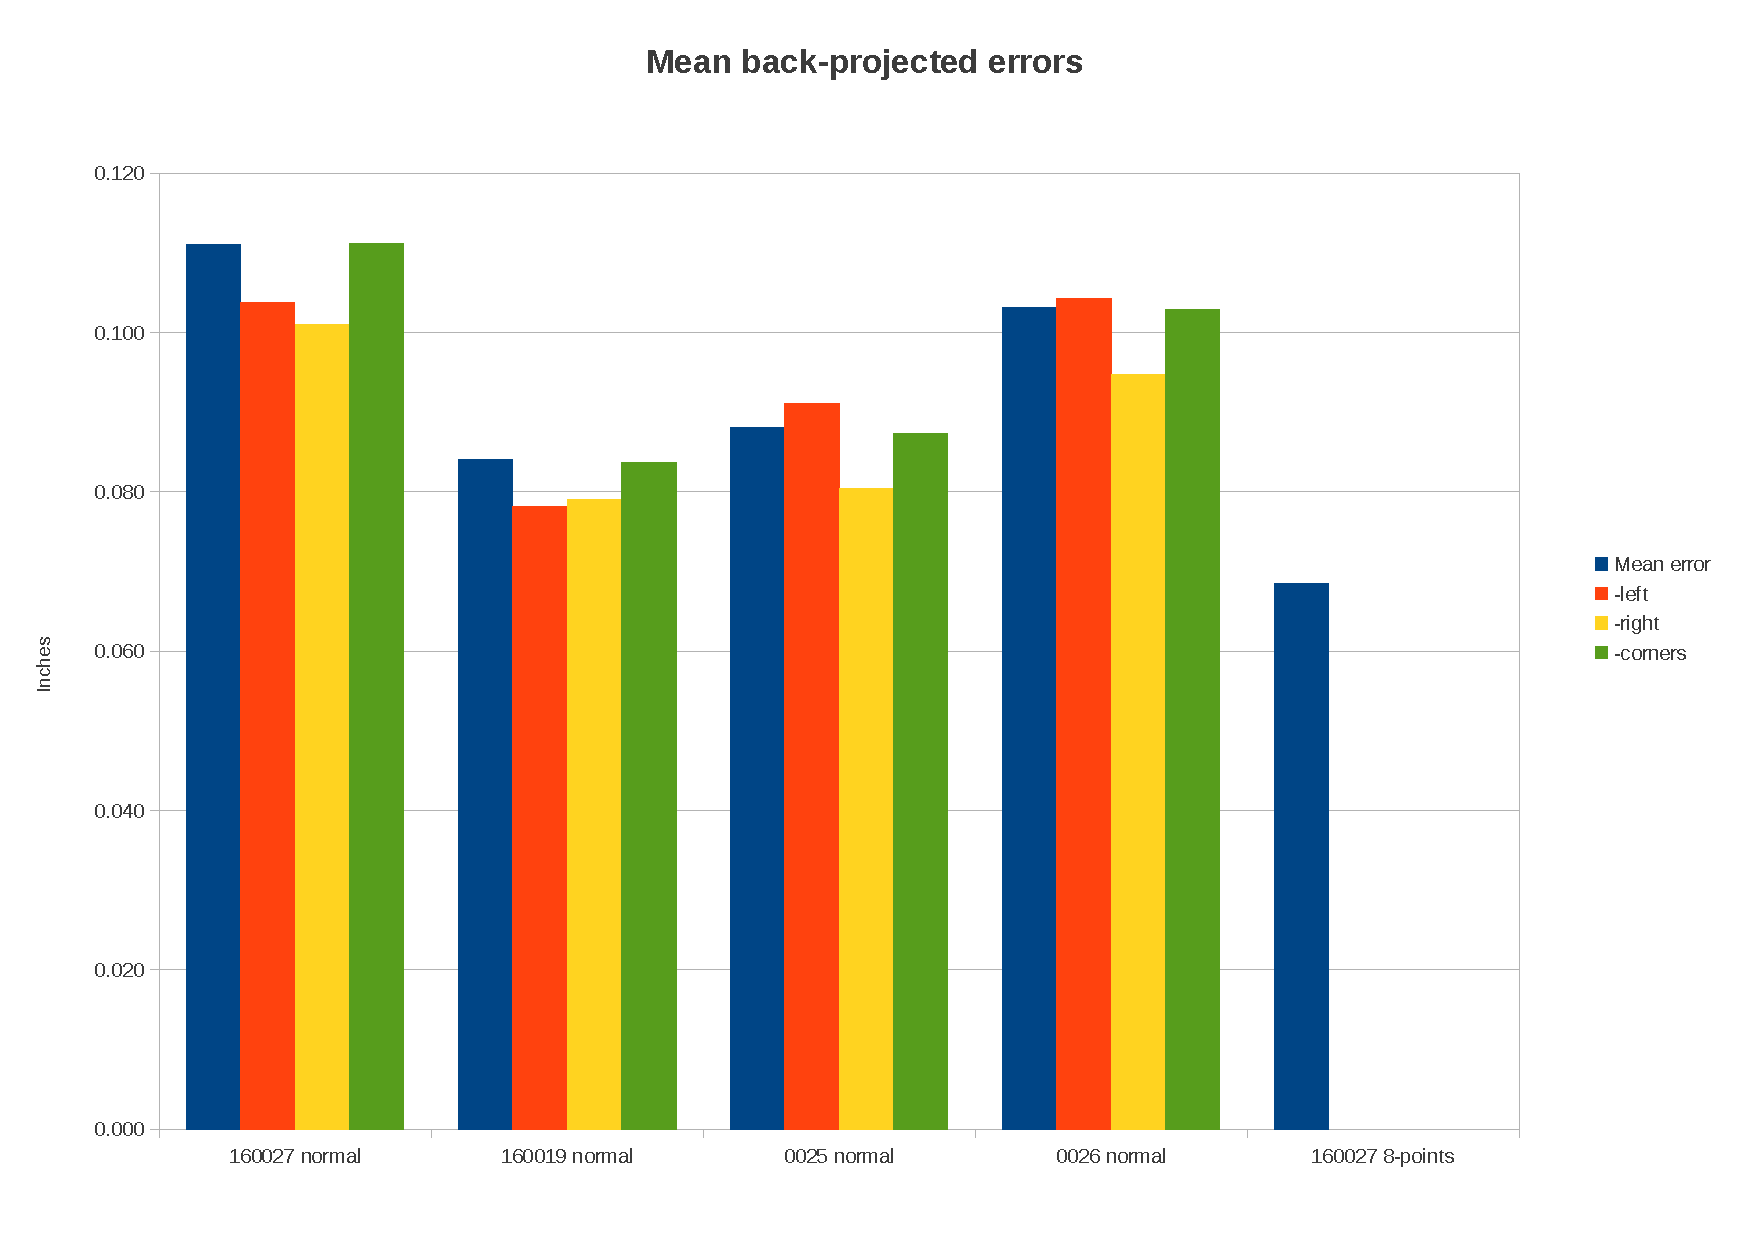
\includegraphics[width=0.7\textwidth]{figures/calibration-means}
  \caption[Mean calibration errors]{Mean calibration errors for all
    calibration points. Each set of bars is from a different image of
    the same calibration object. The images are taken with two
    different cameras, two with each camera. The lone bar on the right
    is the mean error calculated from the first image, but with only
    the 8 centre-most calibration points.}
  \label{fig:calib-errors}
\end{figure}



%Calibration experiments:\\
%
%-> On eight images (2 low grade, 2 high grade, 2 low grade distorted,
%2 high grade distorted)...\\
%
%-> Compare backprojection accuracy... mean, variance, worst hit, best
%hit, breakdown into (x,y,z) \\
%
%-> Compare kappa calculated (should be higher with lens distortion...
%but using actual fisheye distortion may be so high that the polynomial
%kappa model is unsuitable for it, as \cite{straightlines} (I believe
%ot was) suggests can happen).\\
%
%-> Subjectively, look at the resulting translation and rotation
%matrices and consider what they mean, as well as the sx and
%focalLength.\\
%
